\begin{figure*}[tb]
  \centering
  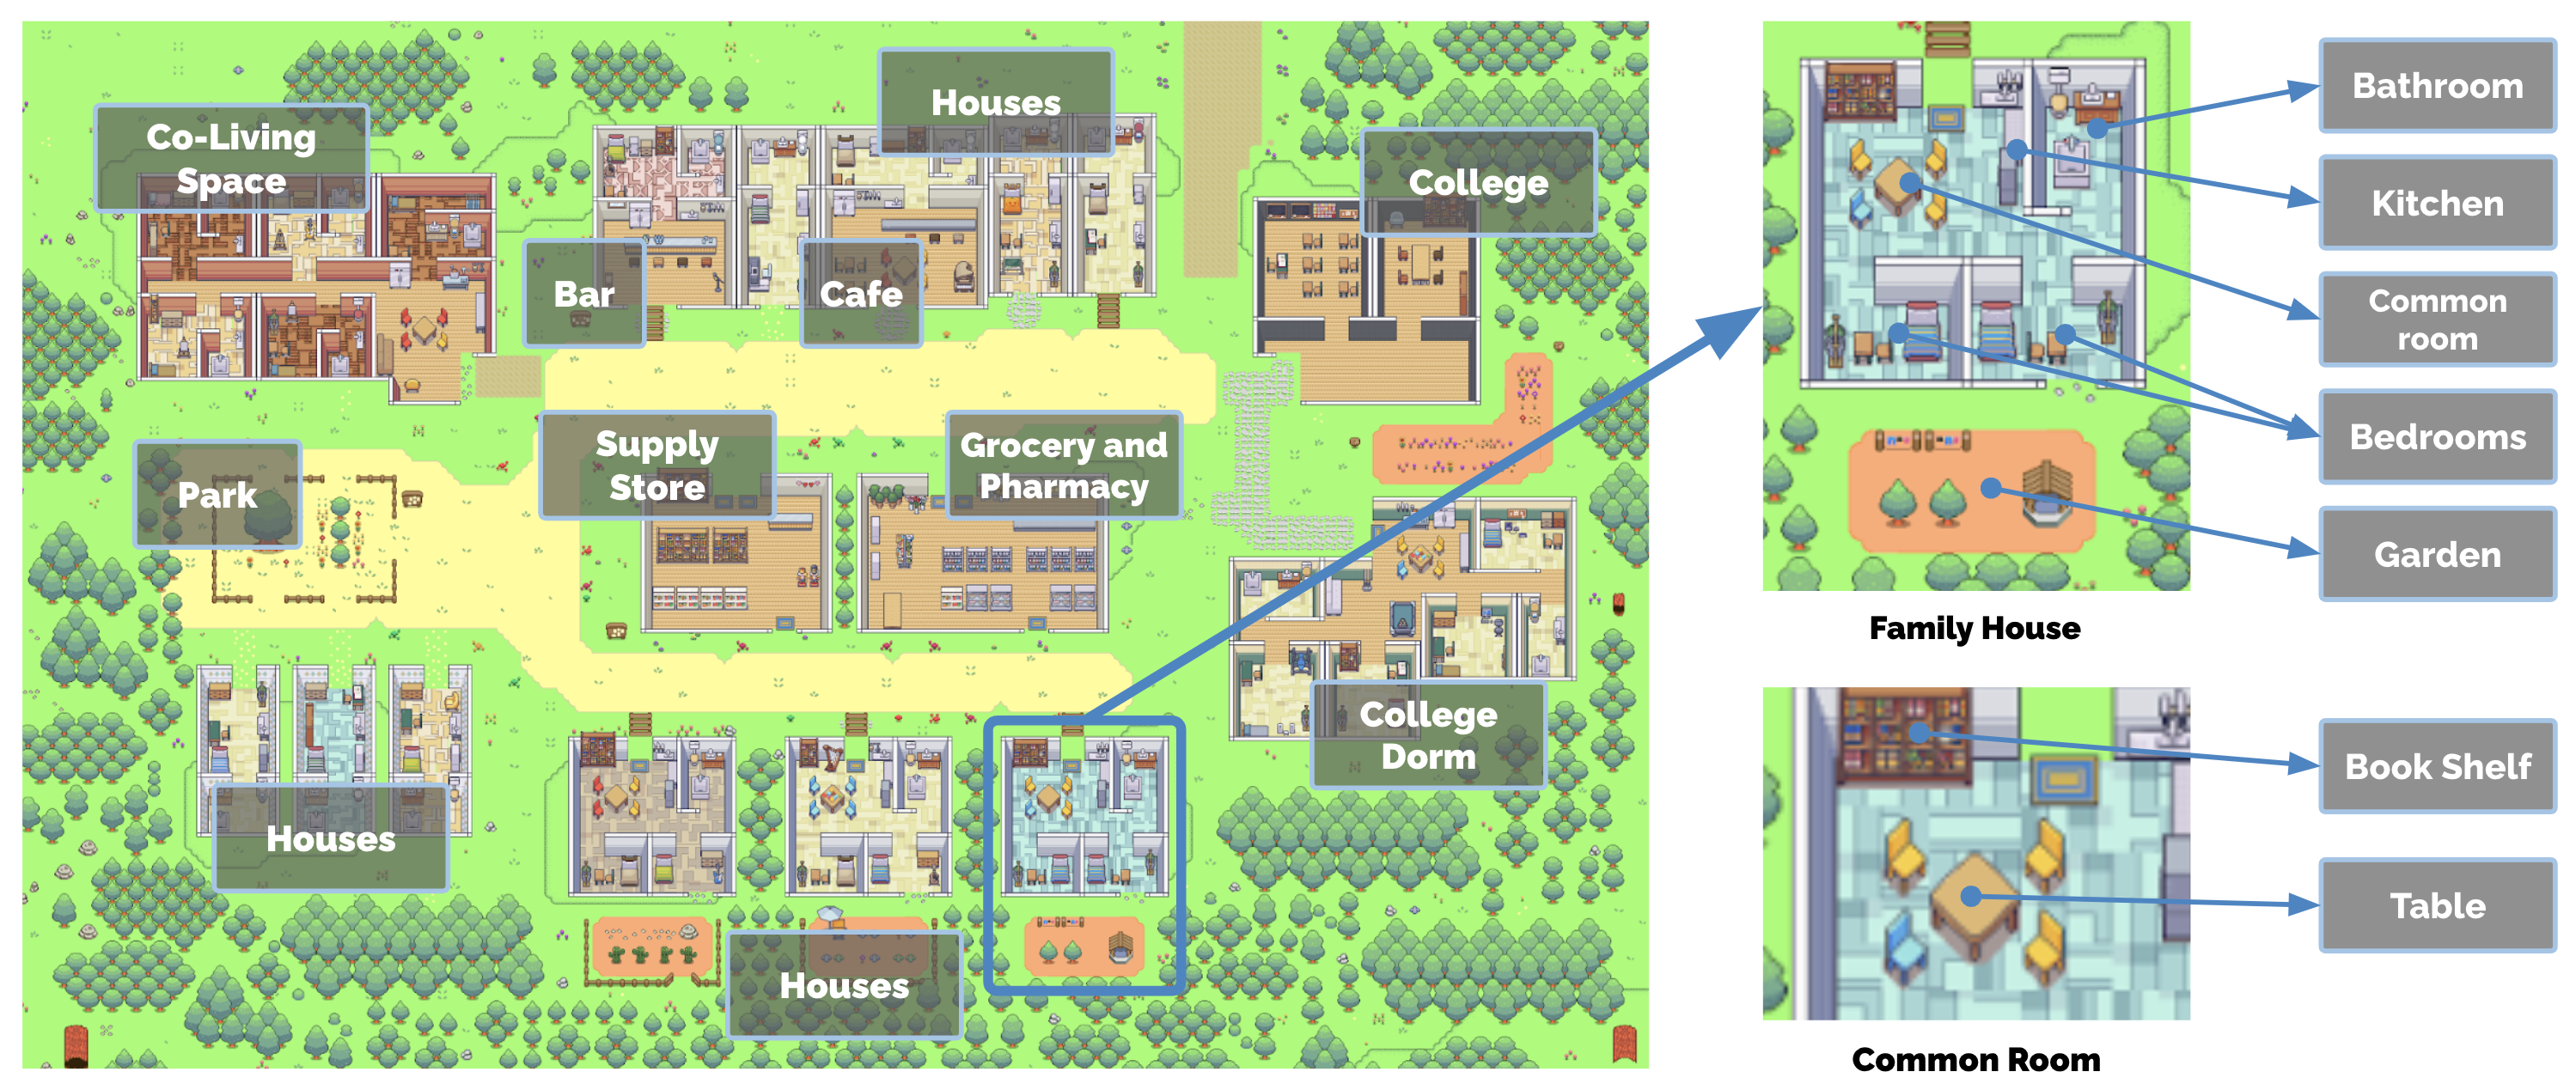
\includegraphics[width=0.98\textwidth]{figures/figure_map5.png}
  \caption{The Smallville sandbox world, with areas labeled. The root node describes the entire world, children describe areas (e.g., houses, cafe, stores), and leaf nodes describe objects (e.g., table, bookshelf). Agents remember a subgraph that reflects the parts of the world they have seen, maintaining the state of those parts as they observed them.}
  \Description{The labeled map of the game world.}
  \label{fig:game_world}
\end{figure*}



\section{Generative Agent Behavior and Interaction}\label{sec:behavior}
To illustrate the affordances of generative agents, we instantiate them as characters in a simple sandbox world reminiscent of The Sims~\cite{49_ElectronicArts2009Sims}. This sprite-based sandbox game world, Smallville, evokes a small town environment. In this section, we will walk through the affordances and interactions with generative agents in Smallville and describe how the agents behave within it. Then, in Section~\ref{sec:architecture}, we will introduce our generative agent architecture that powers these affordances and interactions. In Section~\ref{sec:implementation}, we will describe the implementation of the sandbox environment and how the agents interact with the underlying engine of the sandbox world.

\subsection{Agent Avatar and Communication}\label{sec:avatar}
A community of 25 unique agents inhabits Smallville. Each agent is represented by a simple sprite avatar. We authored one paragraph of natural language description to depict each agent's identity, including their occupation and relationship with other agents, as seed memories. For example, John Lin has the following description:
\begin{quote}
{\small
\texttt{John Lin is a pharmacy shopkeeper at the Willow Market and Pharmacy who loves to help people. He is always looking for ways to make the process of getting medi\-cation easier for his customers; John Lin is living with his wife, Mei Lin, who is a college professor, and son, Eddy Lin, who is a student studying music theory; John Lin loves his family very much; John Lin has known the old couple next-door, Sam Moore and Jennifer Moore, for a few years; John Lin thinks Sam Moore is a kind and nice man; John Lin knows his neighbor, Yuriko Yamamoto, well; John Lin knows of his neighbors, Tamara Taylor and Carmen Ortiz, but has not met them before; John Lin and Tom Moreno are colleagues at The Willows Market and Pharmacy; John Lin and Tom Moreno are friends and like to discuss local politics together; John Lin knows the Moreno family somewhat well — the husband Tom Moreno and the wife Jane Moreno.}
}
\end{quote}
Each semicolon-delimited phrase is entered into the agent's initial memory as memories at the start of the simulation. 

\subsubsection{Inter-Agent Communication}
The agents interact with the world by their actions, and with each other through natural language. At each time step of the sandbox engine, the agents output a natural language statement describing their current action, such as ``Isabella Rodriguez is writing in her journal'', ``Isabella Rodriguez is checking her emails'', ``Isabella Rodriguez is talking with her family on the phone'', or ``Isabella Rodriguez is getting ready for bed.'' This statement is then translated into concrete movements that affect the sandbox world. The action is displayed on the sandbox interface as a set of emojis, providing an abstract representation of the action from an overhead view. To achieve this, the system utilizes a language model to translate the action into a set of emojis, which appear above each avatar's head in a speech bubble. For example, ``Isabella Rodriguez is writing in her journal'' is displayed as \raisebox{-0.1cm}{\protect
\includegraphics[width=0.3cm]{figures/book.png}}\raisebox{-0.1cm}{\protect
\includegraphics[width=0.3cm]{figures/pencil.png}}, while ``Isabella Rodriguez is checking her emails'' appears as \raisebox{-0.1cm}{\protect
\includegraphics[width=0.3cm]{figures/laptop.png}}\,\raisebox{-0.1cm}{\protect
\includegraphics[width=0.3cm]{figures/envelope.png}}. The complete natural language description of the action can be accessed by clicking on the agent's avatar.

Agents communicate with each other in full natural language. They are aware of other agents in their local area, and the generative agent architecture determines whether they walk by or engage in conversation. Here, a sample in the middle of a conversation between the agents Isabella Rodriguez and Tom Moreno about the upcoming election:\footnote{We note that the conversational style of these agents can feel overly formal, likely a result of instruction tuning in the underlying models. We expect that the writing style will be better controllable in future language models.}
\begin{quote}
    \gentxt{
        \textbf{Isabella}: I’m still weighing my options, but I’ve been discussing the election with Sam Moore. What are your thoughts on him? \\
        \textbf{Tom}: To be honest, I don’t like Sam Moore. I think he’s out of touch with the community and doesn’t have our best interests at heart.
    }
\end{quote}

\subsubsection{User Controls}
The user communicates with the agent through natural language by specifying a persona that the agent should perceive them as. For example, if the user specifies that they are a news ``reporter'' and asks about the upcoming election by saying, ``Who is running for office?'', the John agent replies:
\begin{quote}
    \gentxt{
        \textbf{John}: My friends Yuriko, Tom and I have been talking about the upcoming election and discussing the candidate Sam Moore. We have all agreed to vote for him because we like his platform.
    }
\end{quote}
To directly command one of the agents, the user takes on the persona of the agent’s ``inner voice''---this makes the agent more likely to treat the statement as a directive. For instance, when told “You are going to run against Sam in the upcoming election” by a user as John's inner voice, John decides to run in the election and shares his candidacy with his wife and son.

\subsection{Environmental Interaction}
Smallville features the common affordances of a small village, including a cafe, bar, park, school, dorm, houses, and stores. It also defines subareas and objects that make those spaces functional, such as a kitchen in a house and a stove in the kitchen (Figure~\ref{fig:game_world}). All spaces serving as agents’ primary living quarters feature a bed, desk, closet, shelf, as well as a bathroom and a kitchen.\footnote{This environment design is not the focus of our work, so we generated this environment manually, not automatically. Future work can continue to expand the richness of the agents' environments.}

Agents move around Smallville as one would in a simple video game, entering and leaving buildings, navigating its map, and approaching other agents. Agent movements are directed by the generative agent architecture and the sandbox game engine: when the model dictates that the agent will move to a location, we calculate a walking path to the destination in the Smallville environment, and the agent begins moving. In addition, users can also enter the sandbox world of Smallville as an agent operating within it. The agent that the user embodies can be an agent already present in the world, such as Isabella and John, or it can be an outside visitor with no prior history in Smallville. The inhabitants of Smallville will treat the user-controlled agent no differently than they treat each other. They recognize its presence, initiate interactions, and remember its behavior before forming opinions about it.

Users and agents can influence the state of the objects in this world, much like in sandbox games such as The Sims. For example, a bed can be occupied when an agent is sleeping, and a refrigerator can be empty when an agent uses up the ingredients to make breakfast. End users can also reshape an agent's environment in Smallville by rewriting the status of objects surrounding the agent in natural language. For instance, when Isabella is making breakfast in the morning, the user can change the status of the kitchen stove from “turned on” to “burning” by inputting a command to the system that chooses the object and illustrates its new status, like this: ``<Isabella's apartment: kitchen: stove> is burning.'' Isabella will notice this in the next moment and go to turn off the stove and remake her breakfast. Likewise, if the user sets the status of Isabella's shower to “leaking water” when she enters the bathroom, she will gather tools from her living room and try to fix the leak. 

\begin{figure*}[tb]
  \centering
  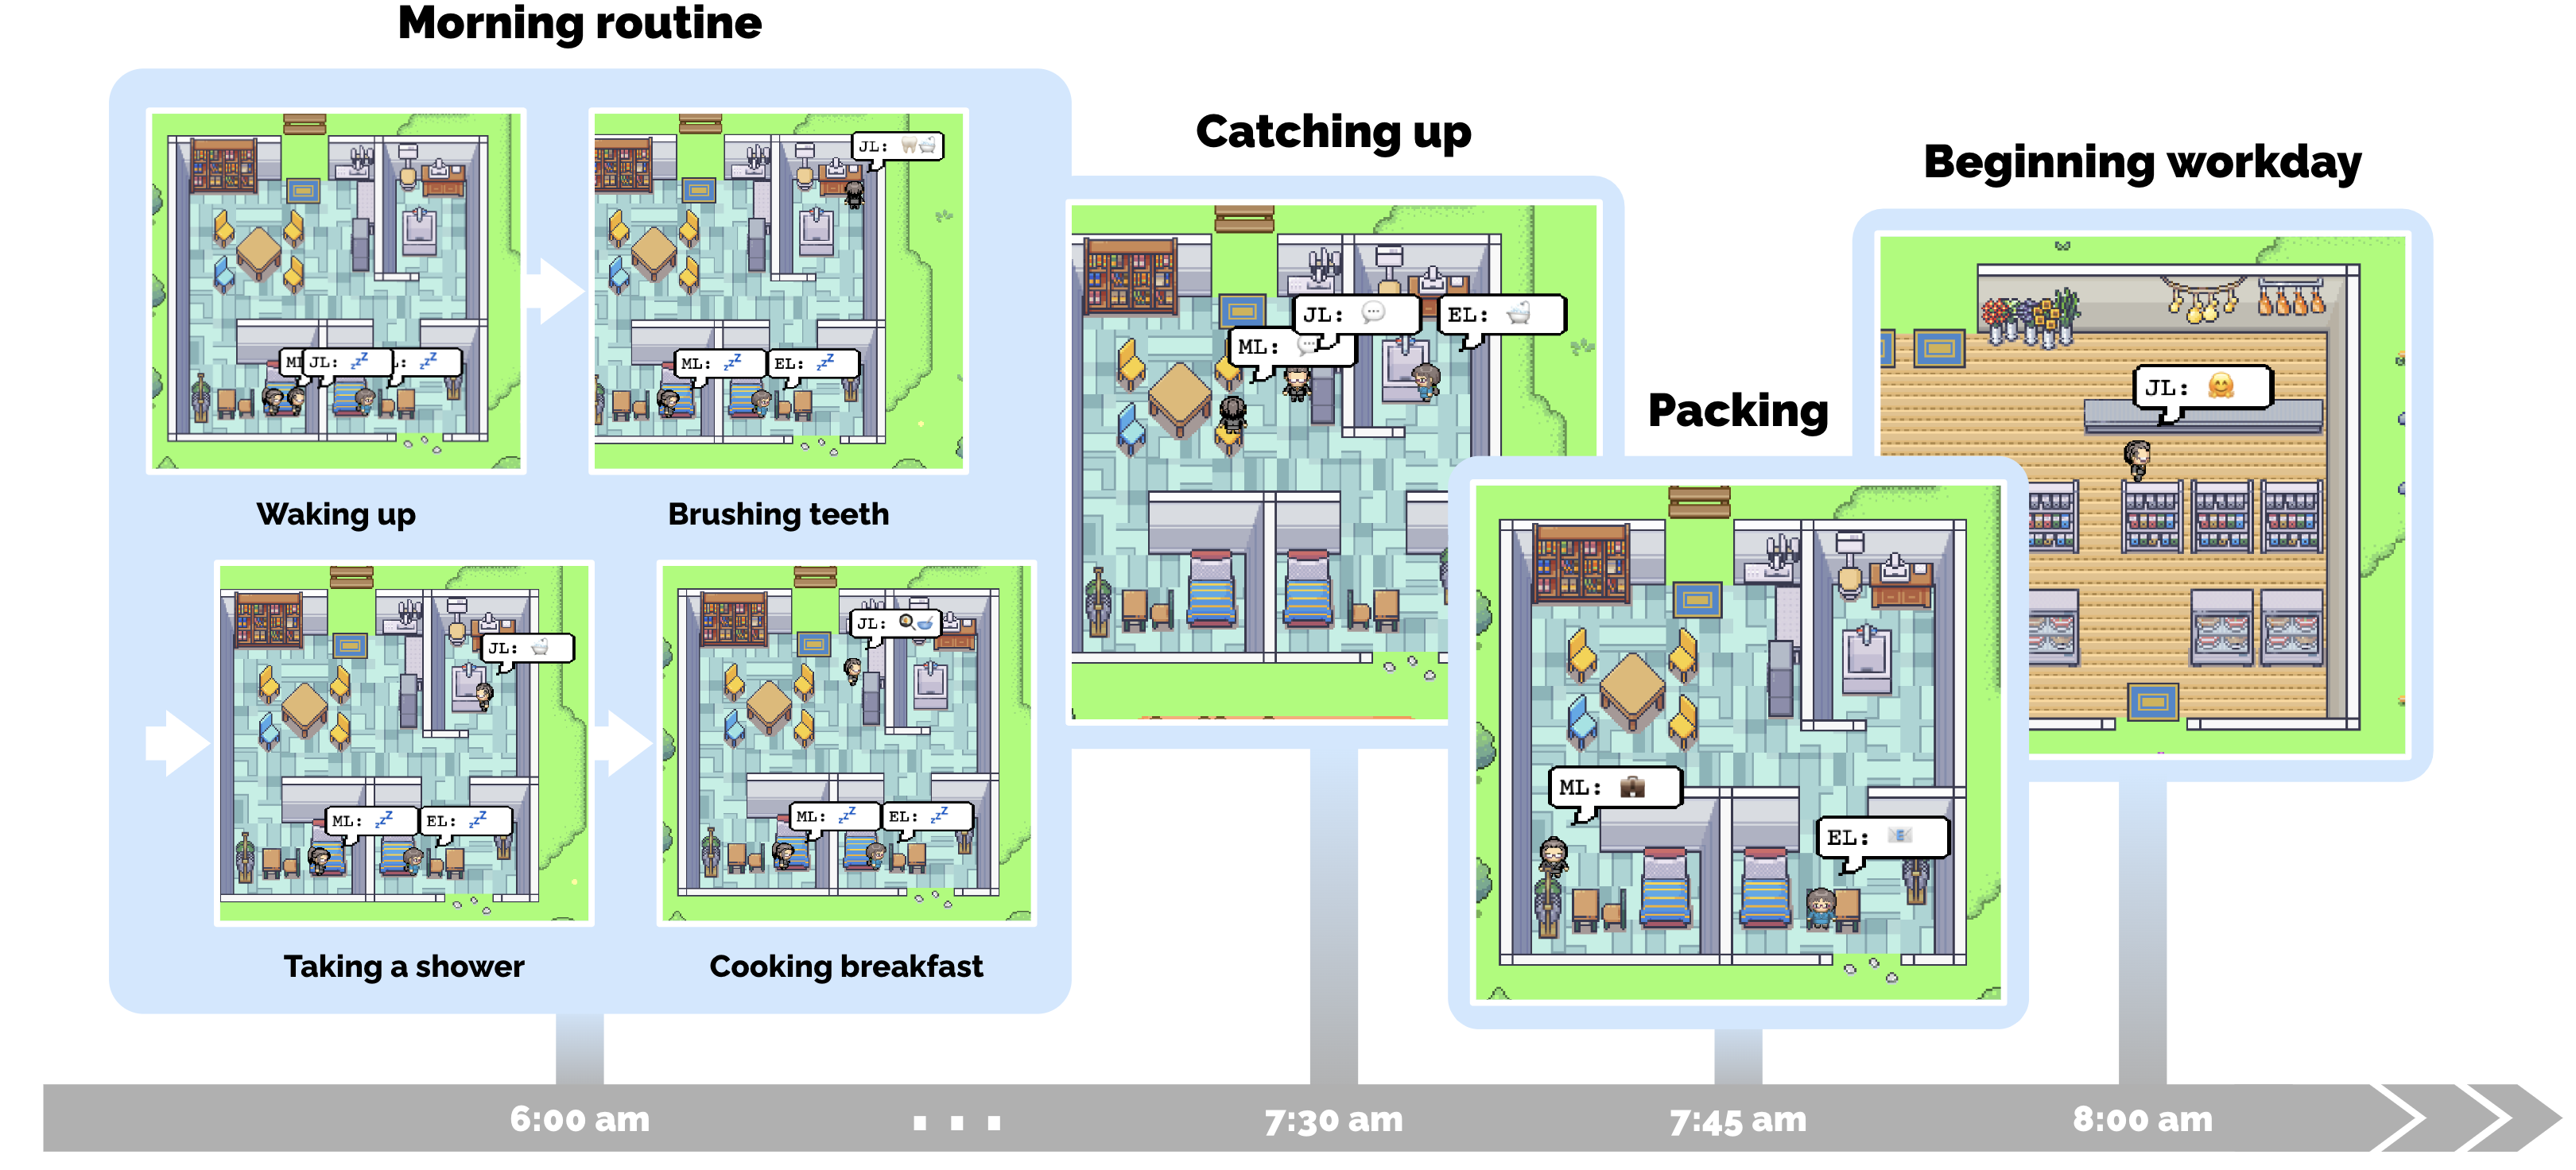
\includegraphics[width=0.95\textwidth]{figures/figure_daily_routine3.png}
  \caption{A morning in the life of a generative agent, John Lin. John wakes up around 6 am and completes his morning routine, which includes brushing his teeth, taking a shower, and eating breakfast. He briefly catches up with his wife, Mei, and son, Eddy, before heading out to begin his workday.}
  \Description{The Lin family's morning routines.}
  \label{fig:Lin_family_morning}
\end{figure*}



\begin{figure}[tb]
  \centering
  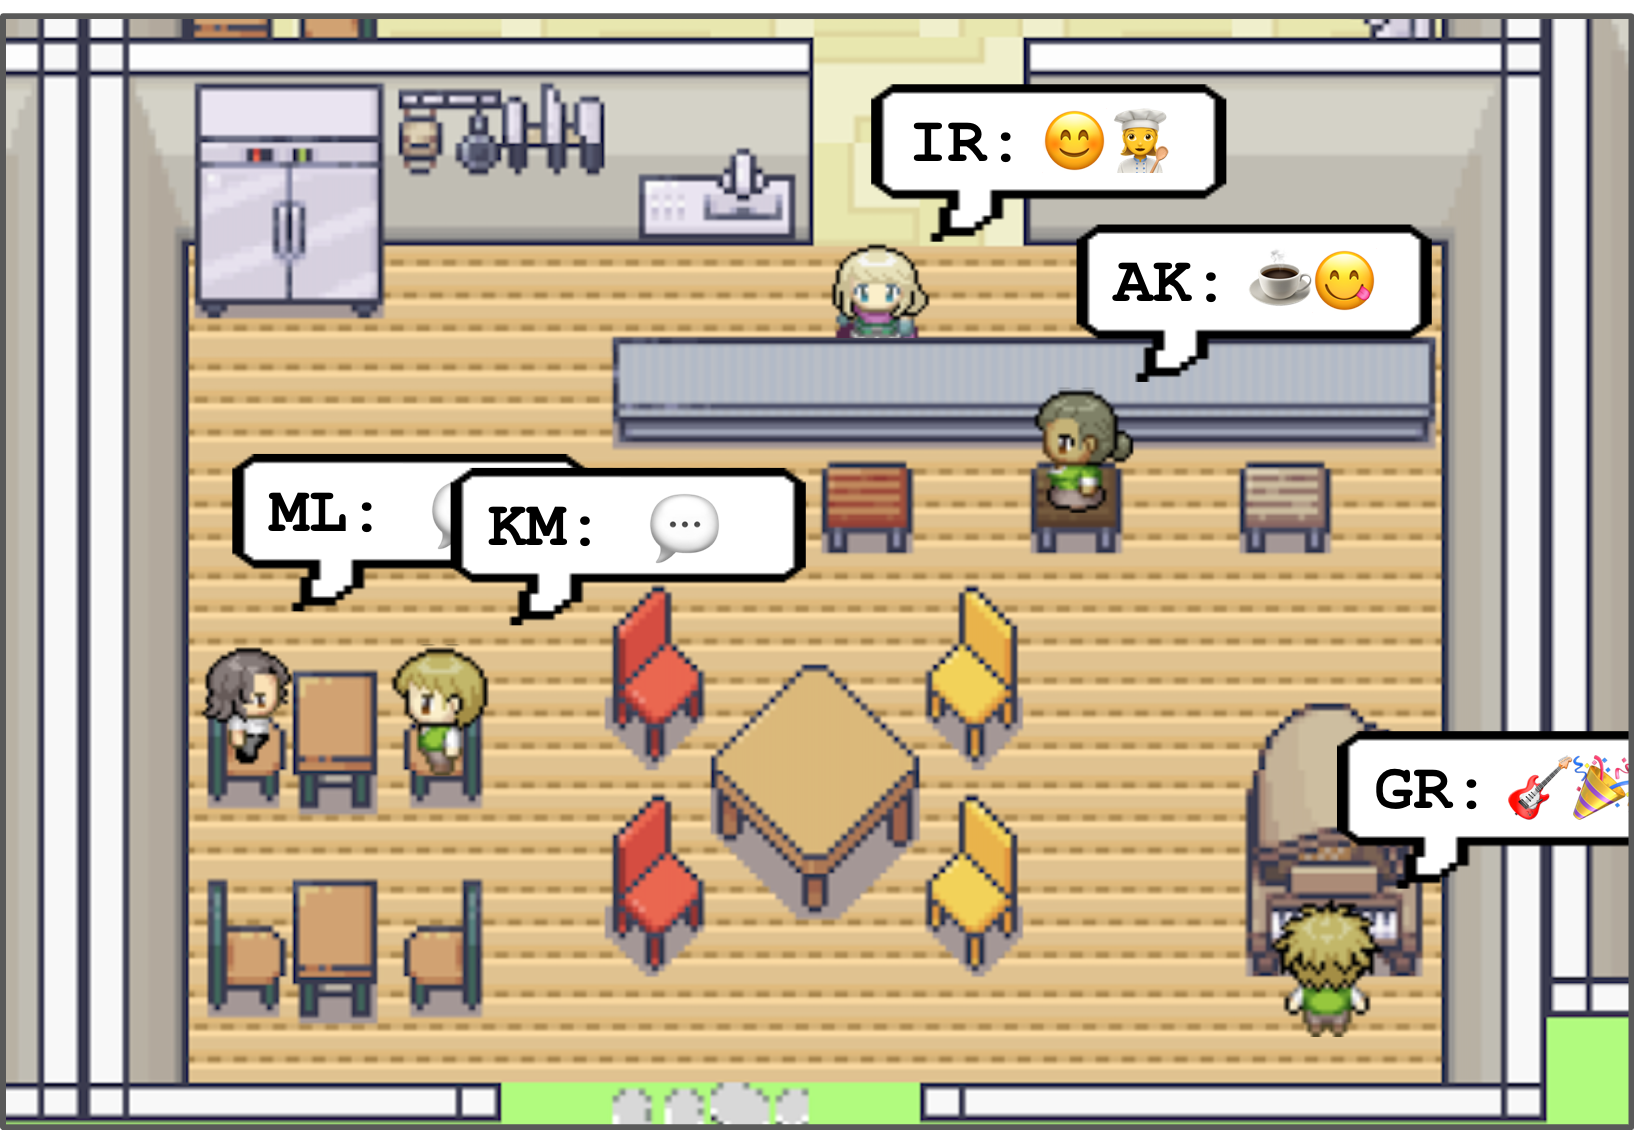
\includegraphics[width=0.75\columnwidth]{figures/figure_valentine3.png}
  \caption{At the beginning of the simulation, one agent is initialized with an intent to organize a Valentine's Day party. Despite many possible points of failure in the ensuing chain of events---agents might not act on that intent, might forget to tell others, might not remember to show up---the Valentine's Day party does, in fact, occur, with a number of agents gathering and interacting.}
  \Description{The Valentine's day party at Hobbs Cafe.}
  \label{fig:valentine}
\end{figure}


\subsection{Example ``Day in the Life''}
Starting from the single-paragraph description, generative agents begin planning their days. As time passes in the sandbox world, their behaviors evolve as these agents interact with each other and the world, building memories and relationships, and coordinating joint activities.

We demonstrate the behavior of generative agents by tracing the output of our system over the course of one day for the agent John Lin (Figure~\ref{fig:Lin_family_morning}). In the Lin family, John is the first to wake up at 7 a.m. He brushes his teeth, takes a shower, gets dressed, eats breakfast, and checks the news at the dining table in the living room. At 8 a.m., Eddy follows suit, rushing out of bed to prepare for his classes. He catches up with John just as he is about to head out:
\begin{quote}
    \gentxt{
        \textbf{John}: Good morning Eddy. Did you sleep well? \\
        \textbf{Eddy}: Good morning dad. Yeah, I slept great. \\
        \textbf{John}: That's good. What are you working on today? \\
        \textbf{Eddy}: I'm working on a new music composition for my class. It's due this week, so I'm trying to get it finished. But I'm having so much fun with it! \\
        \textbf{John}: That sounds great!}  
\end{quote}
Soon after Eddy heads out, Mei wakes up and joins John. Mei asks about her son, and John recalls the conversation they just had:
\begin{quote}
    \gentxt{
        \textbf{Mei}: Did Eddy already leave for school? \\
        \textbf{John}: Yes, he just left. He's working on a music composition for his class. \\
        \textbf{Mei}: Oh, that's wonderful! Tell me about it. \\
        \textbf{John}: I think he's really enjoying it! He said he's having a lot of fun with it. \\
        \textbf{Mei}: That's great! I'm so proud of him.
    }
\end{quote}
As they finish their conversation, Mei and John pack up. Mei goes on to teach and work on her research paper, while John opens his pharmacy counter at the Willow Market and Pharmacy by 9 a.m. 

\begin{figure*}[tb]
  \centering
  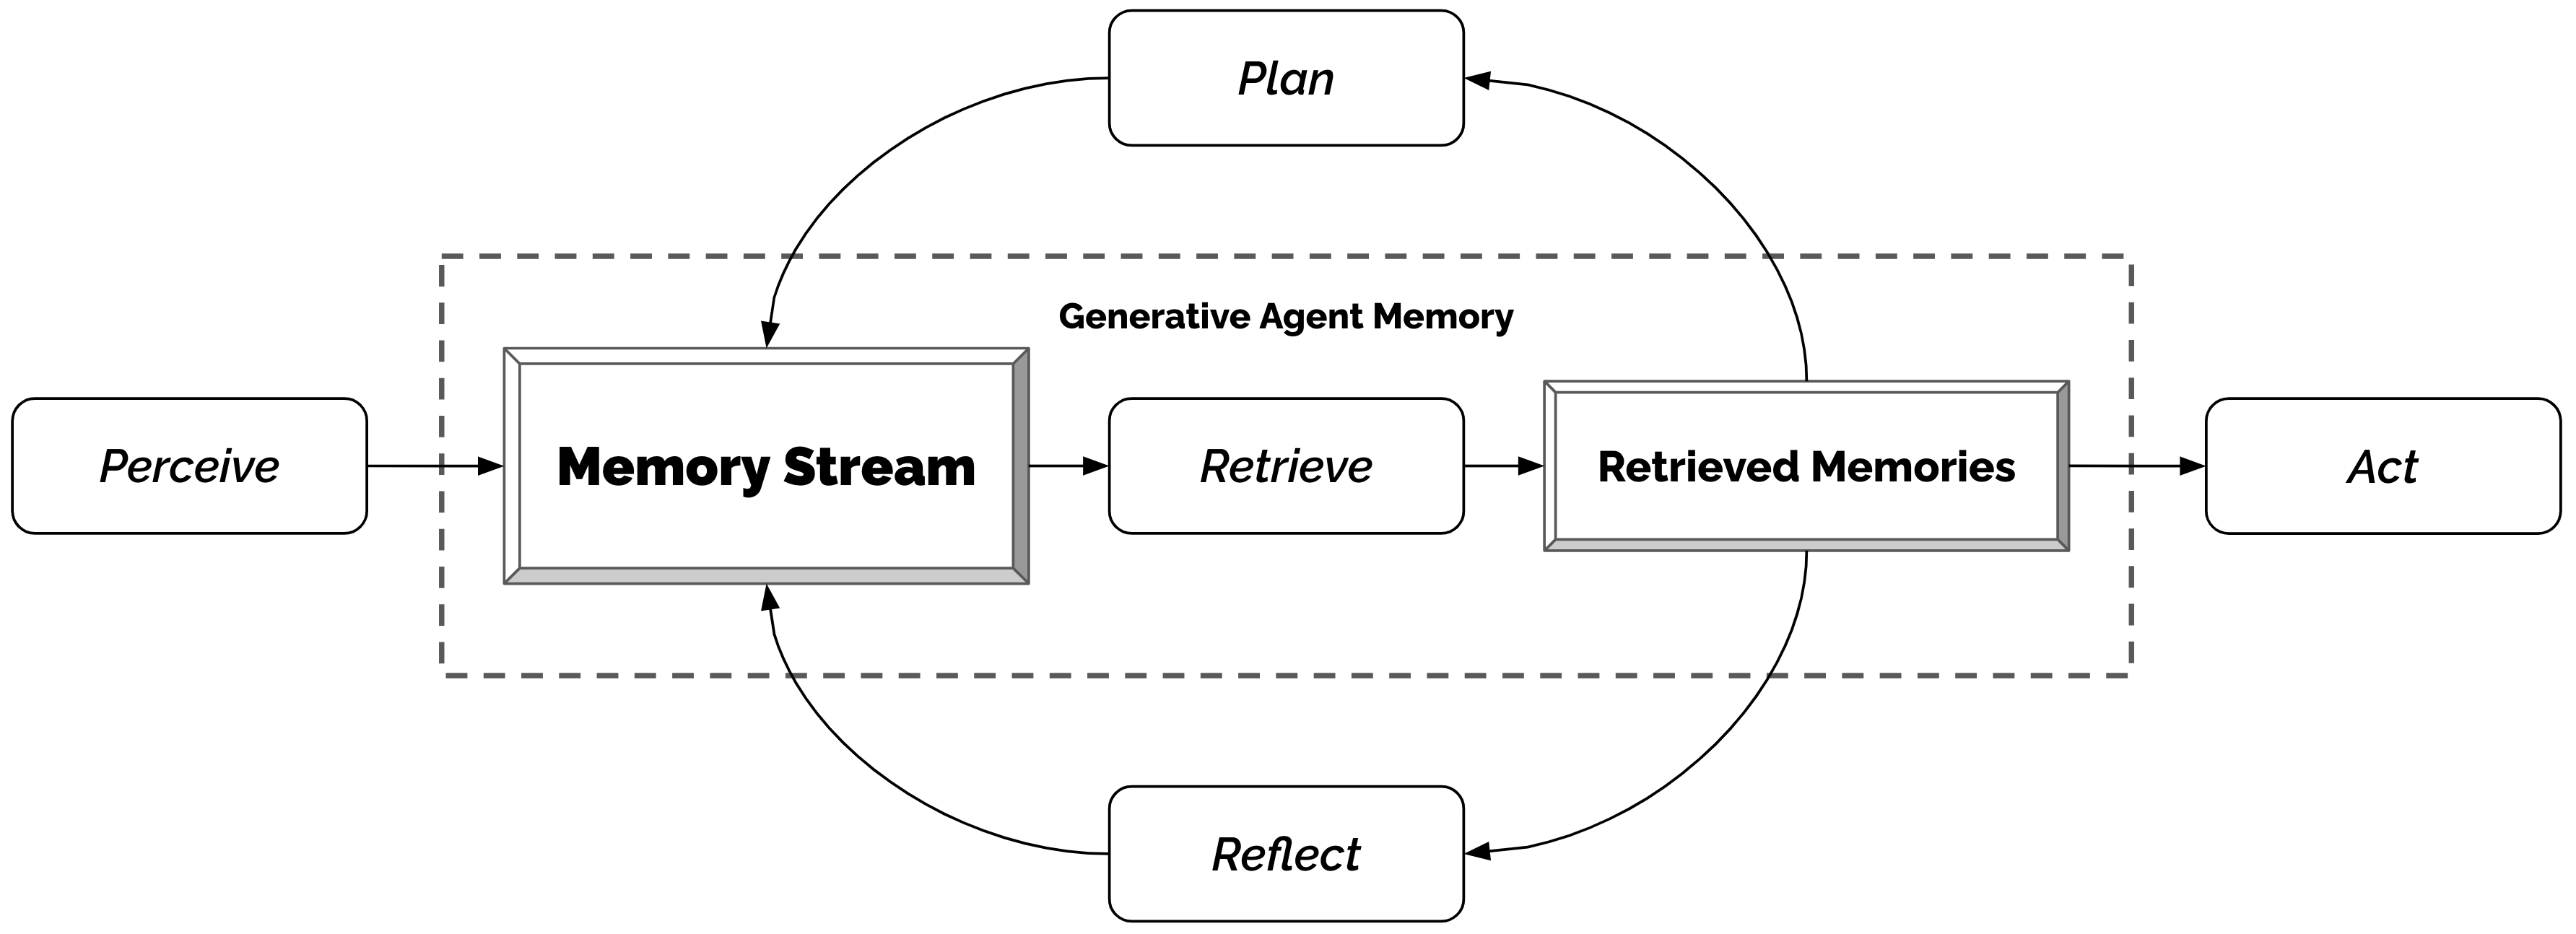
\includegraphics[width=0.88\textwidth]{figures/figure_architecture2.png}
  \caption{Our generative agent architecture. Agents perceive their environment, and all perceptions are saved in a comprehensive record of the agent's experiences called the memory stream. Based on their perceptions, the architecture retrieves relevant memories and uses those retrieved actions to determine an action. These retrieved memories are also used to form longer-term plans and create higher-level reflections, both of which are entered into the memory stream for future use.}
  \Description{The architecture of generative agents.}
  \label{fig:architecture}
\end{figure*}




\subsection{Emergent Social Behaviors}
By interacting with each other, generative agents in Smallville exchange information, form new relationships, and coordinate joint activities. Extending prior work~\cite{9_park2022socialsimulacra}, these social behaviors are emergent rather than pre-programmed. 

\subsubsection{Information Diffusion} 
As agents notice each other, they may engage in dialogue---as they do so, information can spread from agent to agent. For instance, in a conversation between Sam and Tom at the grocery store, Sam tells Tom about his candidacy in the local election:
\begin{quote}
    \gentxt{
        \textbf{Sam}: Hey Tom, how's it going? \\
        \textbf{Tom}: Good, thanks. What's up? \\
        \textbf{Sam}: Well, I wanted to talk to you about something. I'm actually running for mayor in the upcoming local election. \\
        \textbf{Tom}: Really? That's great news! Why are you running? \\
        \textbf{Sam}: I've been involved in local politics for years now, and I really feel like I can make a difference in our community. Plus, I want to bring new ideas and perspectives to the table. 
    }
\end{quote}
Later that day, after Sam left, Tom and John, who heard the news from another source, discuss Sam's chances of winning the election:
\begin{quote}
    \gentxt{
        \textbf{John}: I heard that Sam Moore is running for mayor in the local election. Do you think he has a good chance of winning? \\
        \textbf{Tom}: I do think he has a good chance. He's been working hard in the community and I think he will get a lot of support. What do you think? \\
        \textbf{John}: I think it's great that he's running. I'm curious to see how the election will turn out.
    }
\end{quote}
Gradually, Sam's candidacy becomes the talk of the town, with some supporting him and others remaining undecided. 

\subsubsection{Relationship Memory} 
Agents in Smallville form new relationships over time and remember their interactions with other agents. For example, at the start, Sam does not know Latoya Williams. While taking a walk in Johnson Park, Sam runs into Latoya, and they introduce themselves. Latoya mentions that she is working on a photography project: \gentxt{``I'm here to take some photos for a project I'm working on.''} In a later interaction, Sam's interactions with Latoya indicate a memory of that interaction, as he asks \gentxt{``Hi, Latoya. How is your project going?''} and she replies \gentxt{``Hi, Sam. It’s going well!''}

\subsubsection{Coordination} 
Generative agents coordinate with each other. Isabella Rodriguez, at Hobbs Cafe, is initialized with an intent to plan a Valentine's Day party from 5 to 7 p.m. on February 14th. From this seed, the agent proceeds to invite friends and customers when she sees them at Hobbs Cafe or elsewhere. Isabella then spends the afternoon of the 13th decorating the cafe for the occasion. Maria, a frequent customer and close friend of Isabella's, arrives at the cafe. Isabella asks for Maria's help in decorating for the party, and Maria agrees. Maria's character description mentions that she has a crush on Klaus. That night, Maria invites Klaus, her secret crush, to join her at the party, and he gladly accepts.

On Valentine's Day, five agents, including Klaus and Maria, show up at Hobbs Cafe at 5 pm, and they enjoy the festivities (Figure~\ref{fig:valentine}). In this scenario, the end user only set Isabella's initial intent to throw a party and Maria's crush on Klaus: the social behaviors of spreading the word, decorating, asking each other out, arriving at the party, and interacting with each other at the party were initiated by the agent architecture.

